%!TEX root = ../dissertation.tex

\chapter{Research Proposal}
\label{chapter:researchproposal}
In this section, we introduce the majority of topics to be further studied, the different phases of our research, the metrics we are going to collect and how we are going to treat them. Since we aim to \emph{study to what extent can a user distinguish different amounts of blended colors, when using color mixtures to convey information}, it is important learn from previous results, testing out not only the validity of them but also some missed opportunities. \par
There are several aspects to be considered when developing the broadest study possible: regarding color blending profiling tests, it exists - among
others - some questions which remain unanswered; some of them were risen in the studies by Gama and Gonçalves \cite{Gama20141,Gama20142}. These questions can be divided in four categories:
%
\begin{itemize}
	\setlength\itemsep{0.1em}
	\item \textbf{Questions raised Before}
    \begin{itemize}
    	\setlength\itemsep{0.1em}
		\item Will perceived colors correspond to a particular fixed angular value, in the color wheel?
        \item Which is the best formula to blend colors, in each color model? Is it linear interpolation or another?
        \item In the case in which 3 colors are blended, do observers realize all colors at the same time or do they decompose the mixture, firstly in a mixture of two colors and then a blending of a third color?
        \item What is the best way to present color, without influencing color perception?
        \item Does the user \emph{really} understands which colors are involved in a mixing?
	\end{itemize}
    \item \textbf{Perception Questions}
    \begin{itemize}
    	\setlength\itemsep{0.1em}
    	\item Does the order in which colors are mixed, influence mental mixing models? Are there common patterns among mixing orders?
        \item Do shapes and proximity, influence how color is perceived?
        \item Until which extent does background influence the perception of a subject, in particular a blended color?
        \item If color parameters like Saturation, Value or Luminance change in a blending, does it modify color blending perception?
    \end{itemize}
\end{itemize}
\begin{itemize}
    \newpage
    \item \textbf{Information Visualization Questions}
    \begin{itemize}
    	\setlength\itemsep{0.1em}
		\item Do continuous scales yield better results than discrete color scales?
        \item What is the influence of nominal color scales in perception?
        \item What are the results if no color scale is presented to guide the user?
	\end{itemize}
    \item \textbf{Cultural Questions}
    \begin{itemize}
    	\setlength\itemsep{0.1em}
		\item Does the gender really influences how the color is perceived? Is it possible to observe a significant gap between male and female answers?
\item Is it possible to observe significant differences in observation, depending on user's cultural background?
	\end{itemize}
\end{itemize} \par
%
Although there are these questions whose answers remains to be found, only a portion of them will meet their answers, since this is Master Thesis Research Problem. However, there is a set of these questions which was considered crucial and, consequently, had more priority above others: it was this set which was the focus of our studies. We intended to perform \textbf{three studies} and, in the following sections, it is covered the entire proposal for the first study, the conditions in which the study is ideally performed and other important details.
%
\section{Study Overview}
\label{sec:studyoverview}
%
As previously referred, only a set of questions is answered in our research. The \textbf{goals for the User Study} are as follows:
%
\begin{itemize}
	\item Study one way to present color which does not influence color perception.
  \item Understand if there is any psychological organization of color, when detailing color mixtures' components.
  \item If possible, obtain results to ascertain the cultural influence in color perception.
  \item Study the influence of discrete and continuous color scales.
\end{itemize}
%
Additionally, it is relevant to understand which color model stands as the best to mix colors which are, from a perceptual point of view, more similar to the users expectation. \par

We have planned to develop this study in three different strands: in a \textbf{Laboratory Environment} (which will allow us to calibrate and perfectly control the entire study conditions), in an \textbf{Online Environment} (which will allow us to disseminate our study to a larger set of users, even without controlling the calibration of the testing environment) and, finally, using \textbf{Mechanical Turk Environment} (Amazon's worldwide crowdsourcing marketplace to perform Human Intelligence Tasks, which we would use in order to acquire a huge set of users, even though we can be dealing with speed-clicker users and letting go almost all environmental control). \par
%
To meet these study requirements, we drafted our study into three different phases: a \textbf{User Profiling Phase}, a \textbf{Calibration Phase}, a \textbf{Color Deficiency Test Phase} and finally, the \textbf{Core Phase}. In the following sections, we detail each of these sections. \par
%
\subsection{User Profiling Phase}
\label{sec:researchprop_userprofiling}
%
In this phase of the study, questions about the Age, Gender, Academic Degree, Nationality, Country of Residence and the Native Language of the user should be asked: these questions will help us conceiving user profiles with key indicators about cultural background and gender relation to results of each test. \par
%
\textbf{\underline{\emph{(... ACRESCENTAR AQUI MAIS INFOS RELEVANTES ...)}}} \par
%
When this phase is concluded, the user will be guided to another stage of the study, to perform the \textbf{Calibration Phase}, where he will be asked to analyze a set of images and answer a pair of questions. \par
%
\subsection{Calibration Phase}
\label{sec:researchprop_colordeficiency}
%
Performing online tests - specially when trying to obtain precise values about color - carries obvious problems on how it is guaranteed the results which may appear are, in fact, compliant with certain patterns of
quality, specially color and monitor calibration patterns. \par
%
To overcome this problem, the ideal solution is to develop a system capable of acquiring information about the user's monitor calibration, \emph{e.g.} Brightness, Contrast, RGB Color Balance, Gamma or Saturation, as a pre-step of the study and apply an appropriate calibration when rendering the study's main page. Since we have not found a way to tackle this solution so far, we developed another solution: to present, as pre-step, some calibration images in which the user will have to perform a set of small tasks, indicating us a set of answers; in the end of the test, we have to analyze the answers to verify if they are compliant with a certain pattern of calibration acceptability, determining if the answers of a certain user can be considered true and not misleading. \par
%
\begin{figure}[!ht]
	\centering
  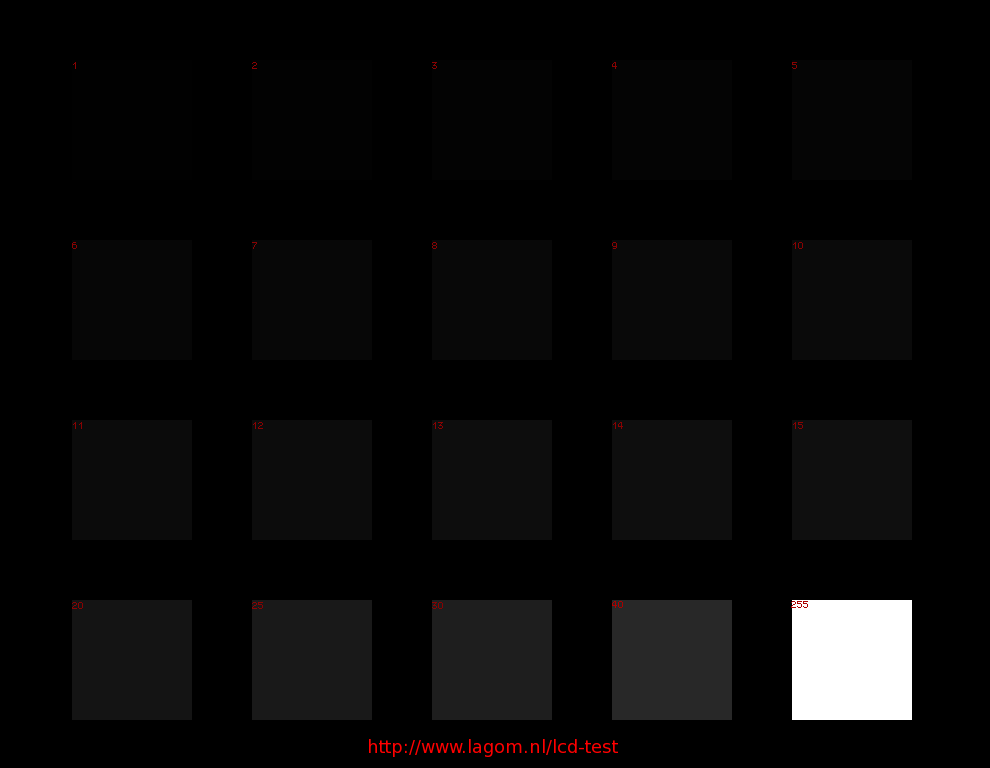
\includegraphics[width=0.35\textwidth]{images/blacktest_example.png}
  \caption[Black Squares Test]{Example of Black Squares Test.\protect\footnotemark{}}
  \label{fig:blacktest_example}
\end{figure}
\footnotetext{"Black Level", Available at: \url{www.lagom.nl/lcd-test/black.php}. Last accessed on September 7th, 2016.}
%
We will present to the user a \textbf{pair of images}, consisting of a set of 10 squares each; in the first of them, we will test the black level of user's monitor, showing each square with a different shade of black, from brighter ones (Square 1) to darker ones (Square 10). The user is, then, asked to express which square is the last, most perceivable, darker square, and point out the word which follows it. The second image has the same job as the first one, except that this rules out the white-level of the monitor and the ten squares present different tones of white. An example of this sort of test is presented in Figure \ref{fig:blacktest_example}. The results of this phase are recorded for further analysis when the study finishes. \par
%
Regarding the laboratory environment, we are going to conduct the user tests in a LCD monitor, under a fixed light source; the monitor will be calibrated
using a colorimeter which will consider the existing light in the environment and adjust the color of each pixel to a standard. The user will be focused on
the task and no other user will be present in the room at the same time, excluding the study regulator; the user will have a fully detailed test protocol to
follow.
%
\textbf{\underline{\emph{(... FALTA TEXTO AQUI ...)}}}
%
\subsection{Color Deficiency Test Phase}
\label{sec:researchprop_colordeficiency}

\subsection{Core Phase}
\label{sec:researchprop_corephase}

\section{User Sample Size}
\label{sec:researchprop_samplesize}

\section{Quality Control}
\label{sec:researchprop_qualitycontrol}

\section{Expected Results}
\label{sec:researchprop_expectedresults}

\section{Time Planning}
\label{sec:background_planning}
